SQL er nokkuð sveigjanlegt og yfirgripsmikið mál. 
Í þessari bók er einungis farið yfir lítið brot af því sem viðfangsefnið hefur upp á að bjóða.

Byrjum á að skoða grundvallaraðgerðirnar í SQL - að búa gagnagrunn, búa til töflur, setja gögn í töflurnar og að skoða gögnin aftur.
\section{Gagnagrunnar}
Fram kom í kafla \ref{kafli:inngangur} að gagnagrunnur sé \emph{skipulagt samansafn af upplýsingum}. Einnig kom fram að upplýsingarnar eru hlutaðar niður með ``töflum''.
\begin{marginfigure}
\caption[Uppbygging gagnagrunns]{Uppbygging einfalds gagnagrunns með þremur töflum.}
\label{mynd:uppbygging-gagnagrunns}
\centering
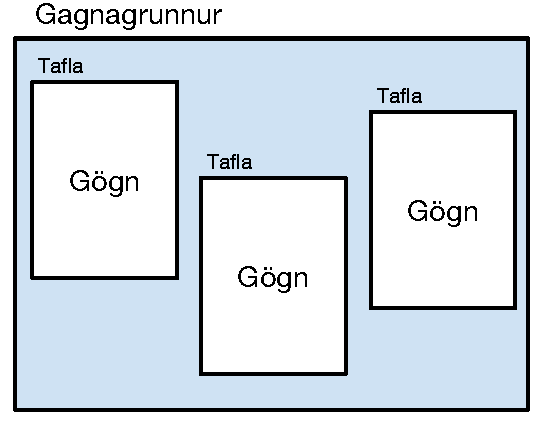
\includegraphics[width=\linewidth]{myndir/uppbygging-gagnagrunns}
\end{marginfigure}
Hér er vert að taka nokkur atriði fram:
\begin{itemize}
 \item Gagnagrunnur er ekki það sama og tölva. Talað er um að gagnagrunnur sé geymdur á tölvu eða jafnvel að tölva keyri gagnagrunns-server. Ein tölva getur geymt marga gagnagrunna.
 \item Gagnagrunnur er ekki forrit. Gagnagrunns\emph{kerfi}\footnote{Sjá undirkafla \ref{undirkafli:gagnagrunnskerfi} og \ref{undirkafli:helstu-gagnagrunnskerfi}}, sem er forrit, keyrir á tölvunni og heldur utan um gagnagrunninn. En gagnagrunnurinn sjálfur er ekki forrit.
\end{itemize}
Líkja mætti gagnagrunni við ``möppu'' í tölvu sem inniheldur töflur\footnote{Reyndar getur gagnagrunnur innihaldið ýmislegt annað en töflur. Slík atriði eru tekin fyrir í seinni áföngum.}. Hægt er að búa til gagnagrunna á tölvu, setja í hann töflur og skoða innihald þeirra.

Við sjáum dæmi um hvernig búa má til gagnagrunn í undirkafla \ref{undirkafli:synidaemi-i-sql}.
\section{Töflur}
Gögn í SQL-gagnagrunni má líta á sem raðir í töflum. Þess vegna er mikilvægt skref í því að læra að nota SQL að vera það að skilja uppbyggingu taflna mjög nákvæmlega.
Lítum fyrst á dæmigerða töflu.

\begin{table}
\centering
\caption[Nokkrir starfsmenn Tækniskólans]{Nokkrir starfsmenn Tækniskólans.}
\label{tafla:starfsmenn-ts}
\begin{tabular}{lll}
\toprule
Nafn&Starfsheiti&Netfang\\
\midrule
Bjargey G. Gísladóttir&Skólastjóri&bbg@tskoli.is\\
Donatas Butkus&Tölvuþjónusta&db@tskoli.is\\
Eiríkur Ernir Þorsteinsson&Kennari&eet@tskoli.is\\
Emil Gautur Emilsson&Kennari&ege@tskoli.is\\
Geir Sigurðsson&Kennari&ges@tskoli.is\\
Gunnar Þórunnarson&Kennari&gus@tskoli.is\\
Guðmundur Jón Guðjónsson&Kennari&gjg@tskoli.is\\
Guðrún Randalín Lárusdóttir&Kennari&grl@tskoli.is\\
Hallur Ó. Karlsson&Kennari&hal@tskoli.is\\
Konráð Guðmundsson&Kennari&kng@tskoli.is\\
Matthias Skúlason&Tölvuþjónusta&matti@tskoli.is\\
Sigurður R. Ragnarsson&Kennari&srr@tskoli.is\\
Snorri Emilsson&Kennari&sem@tskoli.is\\
Tryggvi Jóhannsson&Kerfisstjóri&tj@tskoli.is\\
Þórarinn J. Kristjánsson&Kennari&tjk@tskoli.is\\
\bottomrule
\end{tabular}
\end{table}
Eins og allar alvöru töflur inniheldur þessi starfsmannatafla annars vegar \emph{dálkheiti} og hins vegar \emph{gögn}. Dálkheitin eru ``Nafn'', ``Starfsheiti'' og ``Netfang''. Dæmi um upplýsingar eru að til sé starfsmaður sem heitir ``Eiríkur Ernir Þorsteinsson'', sem er ``Kennari'' og hefur netfangið ``eet@tskoli.is''. 

Mikilvægt er að átta sig á þessum mun - hver einasta tafla sem unnið er með inniheldur dálkheiti og gögn, sem eru aðskilin fyrirbrigði. Þetta á við ``hefðbundnar'' töflur sem við sjáum á prenti og við töflur í forritum á borð við Microsoft Excel. 

En þetta á líka við töflur sem við skilgreinum með SQL-skipunum. SQL-töflur innihalda dálkheiti og gögn, alveg eins og við myndum búast við af hefðbundnum töflum.

Þegar töflur eru sýndar á prenti er venjan að dálkheitin komi fram í fyrstu línu töflunnar (og oftast aðskilin gögnunum með striki). Gögnin koma fram í næstu línum.

Þegar SQL er notað til að lýsa töflum eru dálkheitin og aðrar upplýsingar sem skilgreina töfluna sjálfa búnar til með sérstökum skipunum. Aðrar skipanir eru notaðar til að vinna með gögnin sjálf. Við sjáum dæmi um þessar skipanir í undirkafla \ref{undirkafli:synidaemi-i-sql}. \footnote{Farið í muninn á skipunum sem skilgreina töflur og skipunum sem vinna með gögn í kafla \ref{kafli:uppfaera}.}
\section{Fyrirspurnir}
Ekki er mikið gagn í því að geyma upplýsingar í töfluformi nema að hægt sé að ná í þær aftur.

Einfalt er að fletta upp upplýsingum í litlum töflum á borð við töflu \ref{tafla:starfsmenn-ts} þegar þær eru prentaðar út. Viljum við t.d. komast að því hver er með netfangið ``kng@tskoli.is'' dugar okkur að láta augun reika yfir töfluna þar til við rekumst á netfangið og líta svo í starfsmannadálkinn.

Væri taflan örlítið stærri væri verkefnið strax erfiðara. Væri taflan á stærð við símaskrána væri það nær ómögulegt.

Slíkar uppflettingar, stórar og smáar, eru sérsvið SQL. Þær eru nefndar \emph{fyrirspurnir} og eru framkvæmdar með mjög mikilvægri SQL-skipun sem heitir \emph{SELECT}. Við sjáum dæmi um slíka skipun í næsta undirkafla (\ref{undirkafli:synidaemi-i-sql}) og kynnumst þeim náið í kafla \ref{kafli:select}.

\section{Sýnidæmi í SQL}
\label{undirkafli:synidaemi-i-sql}
Skoðum hvernig búa má til töflu \ref{tafla:starfsmenn-ts} með SQL, setja í hana gögn og sækja gögnin aftur. 

Eins og fram hefur komið þarf að nota SQL-skipanir til þess.

\subsection{Skilgreining gagnagrunns}
Okkar fyrsta verk verður að vera að búa til gagnagrunn til að setja töfluna í. Slíka skipun má sjá á sýnidæmi \ref{sql:k2d4-create-database}.

\begin{example}
\caption{CREATE DATABASE skipun fyrir Tækniskólagagnagrunninn.}
\label{sql:k2d4-create-database}
\centering
\sql{sql/k2d4-create-database.sql}
\end{example}

Skipunin er ein lína. Hér vill reyndar svo til að hún er nálægt því að vera málfræðilega rétt setning á ensku. Hún er einfaldlega lýsing á því sem við viljum að gagnagrunnskerfið geri fyrir okkur: ``búðu til gagnagrunn með nafnið \verb|taekniskolinn|''!

Þetta er mjög einkennandi fyrir SQL. Í SQL erum við nær alltaf að lýsa því \emph{hvað} við viljum gera frekar en \emph{hvernig} við gerum það. Þetta gerir SQL frábrugðið flestum vinsælum forritunarmálum.

\subsection{Skilgreining töflu og innsetning gagna}
Skipunina til að skilgreina töfluna má sjá á SQL-sýnidæmi \ref{sql:k2d1-create-table}. Þetta er mjög dæmigerð skipun til að búa til töflu. Þar kemur fram hvað gera skal (búa til töflu $\rightarrow$ \verb|CREATE TABLE|) og hver dálkheitin eru (nafn, Starfsheiti og netfang). \footnote{Við skulum ekki örvænta þó að skipanirnar séu óskiljanlegar á þessum tímapunkti. Við skoðum skipanirnar vandlega í næsta kafla, þessar eru einungis svo að við getum fengið tilfinningu fyrir því hvernig þær geta litið út.}

\begin{example}[h]
\caption{CREATE TABLE skipun fyrir starfsmannatöfluna.}
\label{sql:k2d1-create-table}
\centering
\sql{sql/k2d1-create-table.sql}
\end{example}

Hér ber að athuga að enn eru engin gögn komin inn í töfluna. Það má gera með skipuninni í SQL-sýnidæmi \ref{sql:k2d2-insert}.

\begin{example}[h]
\caption{INSERT skipun fyrir starfsmannatöfluna.}
\label{sql:k2d2-insert}
\centering
{\small
\sql{sql/k2d2-insert.sql}
}
\end{example}

\subsection{Fyrirspurnir}
Til að sækja gögn úr töflunni þarf síðan að framkvæma fyrirspurn. Dæmi um fyrirspurn (SQL-skipun) sem finnur nafn þess starfsmanns sem er með netfangið ``kng@tskoli.is'' má sjá á sýnidæmi \ref{sql:k2d3-select}.

\begin{example}[h]
\caption{SELECT skipun sem finnur nafnið á þeim kennara sem er með netfangið \emph{kng@tskoli.is}. Það nafn er ``Konráð''.}
\label{sql:k2d3-select}
\centering
\sql{sql/k2d3-select.sql}
\end{example}

Athugum hvað kemur fram í fyrirspurninni. Við getum séð þrjá aðalhluta - lýsingu á því hvað gera skal (finna nafn/\verb|SELECT nafn|), hvaðan upplýsingarnar skulu koma (úr starfsmannatöflunni/\verb|FROM Starfsmenn|) og hvaða \emph{skilyrði} gilda um gögnin sem finna skal (gögnin þar sem netfangið er kng@tskoli.is/\verb|WHERE netfang = "kng@tskoli.is"|). 
\marginnote{Við getum spurt okkur af hverju öll SQL-sýnidæmin eru með sum orðin í hástöfum og af hverju svona fá orð eru í hverri línu. Þetta er vegna þess að 
\begin{enumerate}
 \item Löng hefð er fyrir því að skrifa SQL-lykilorð í hástöfum.
 \item Línubilin eru á þeim stöðum sem höfundi þykir hjálpa mest upp á læsileika.
\end{enumerate}
Hvorugt er strangt til tekið nauðsynlegt.}

\section{Keyrsla í MySQL Workbench}
\label{undirkafli:keyrsla-i-workbench}
Lítum örstutt á hvernig nota má MySQL Workbench til að búa til okkar fyrstu töflu með SQL.

Um nokkur skref er að ræða.
\begin{enumerate}
 \item Ræsa þarf forritið. Við það birtist upphafsskjár, líkur þeim sem sjá má á mynd \ref{mynd:workbench-upphafsskjar}.\footnote{Útlit MySQL Workbench er eðli málsins samkvæmt örlítið mismunandi eftir stýrikerfum og útgáfum á forritinu. Skjáskotin eru tekin af Workbench útgáfu 6.0, á Linux vél.}
 \item Mynda þarf tengingu við MySQL-server. Henni þarf að gefa nafn, IP-tölu MySQL serversins, notandanafn og lykilorð.\footnote{Nemendur Tölvudeildar Tækniskólans skulu biðja kennarann um þessar upplýsingar.} Sjá mynd \ref{mynd:workbench-login}.
 \item Búa þarf til nýjan gagnagrunn á MySQL-servernum á skjánum sem birtist eftir að tengingin er mynduð. Það er gert með \verb|CREATE DATABASE| skipun, sjá mynd \ref{mynd:workbench-create-db}. Þegar þessu er lokið höfum við keyrt okkar fyrstu SQL-skipun!
 \item Skipunin í sýnidæmi \ref{sql:k2d1-create-table} er slegin inn í aðalgluggann og keyrð. Taflan er þá komin inn.
\end{enumerate}
Ávallt má gera ráð fyrir að SQL-sýnidæmi í þessari bók megi keyra með hliðstæðum hætti - í aðalglugga MySQL Workbench. T.d. mætti keyra sýnidæmi \ref{sql:k2d2-insert} og \ref{sql:k2d3-select} á þann hátt.

\begin{figure*}
\caption[Upphafsskjár MySQL Workbench]{Upphafsskjár MySQL Workbench. Örin vísar á hnapp sem nota má til að búa til nýja tengingu.}
\label{mynd:workbench-upphafsskjar}
\centering
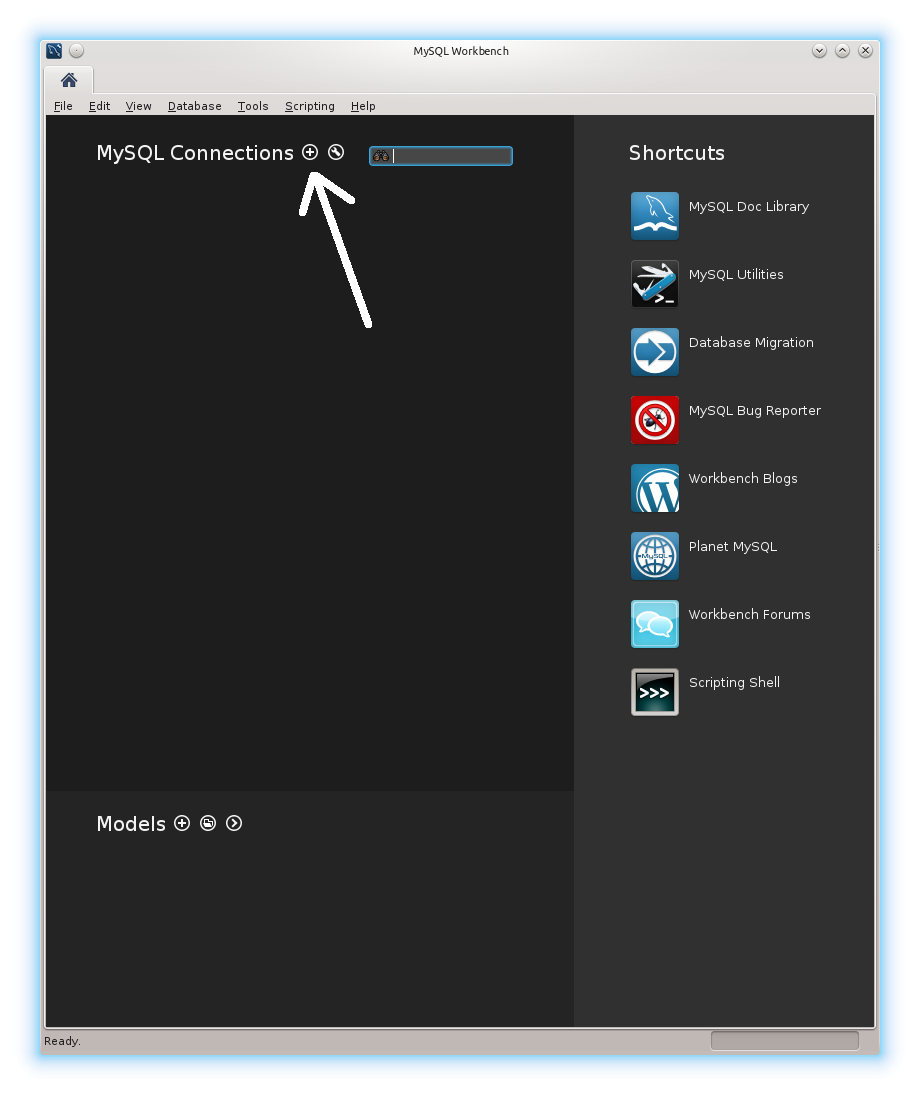
\includegraphics[width=\linewidth]{myndir/workbench-upphafsskjar}
\end{figure*}

\begin{figure*}
\caption[Tengingarskjár MySQL Workbench]{Tengingarskjár MySQL Workbench. Hér er verið að búa til tenginguna ``Prufutenging'', sem tengist MySQL-þjóni sem keyrir á sömu tölvu og Workbench-inn (127.0.0.1) með notandanafninu ``root''.}
\label{mynd:workbench-login}
\centering
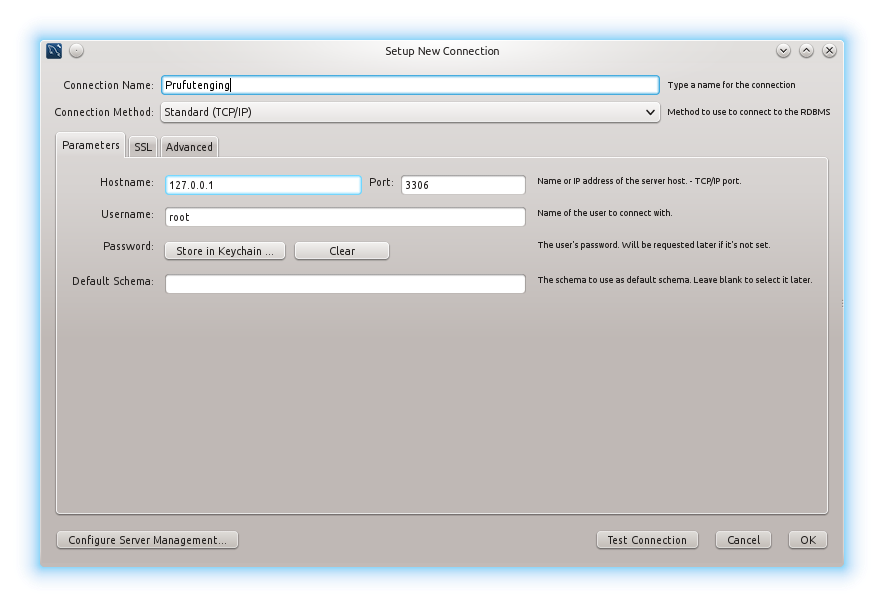
\includegraphics[width=\linewidth]{myndir/workbench-login}
\end{figure*}

\begin{figure*}
\caption[Nýr gagnagrunnur]{Nýr gagnagrunnur búinn til með MySQL Workbench. Efri örin vísar á hnappinn sem ýta þarf á til að keyra SQL-skipunina. Neðri örin vísar á lista af gagnagrunnum sem sýnilegir eru á servernum. Birtist gagnagrunnurinn sem búinn er til ekki um leið og skipunin er keyrð, hægri-smellið þá á listann og ``refresh''ið hann.}
\label{mynd:workbench-create-db}
\centering
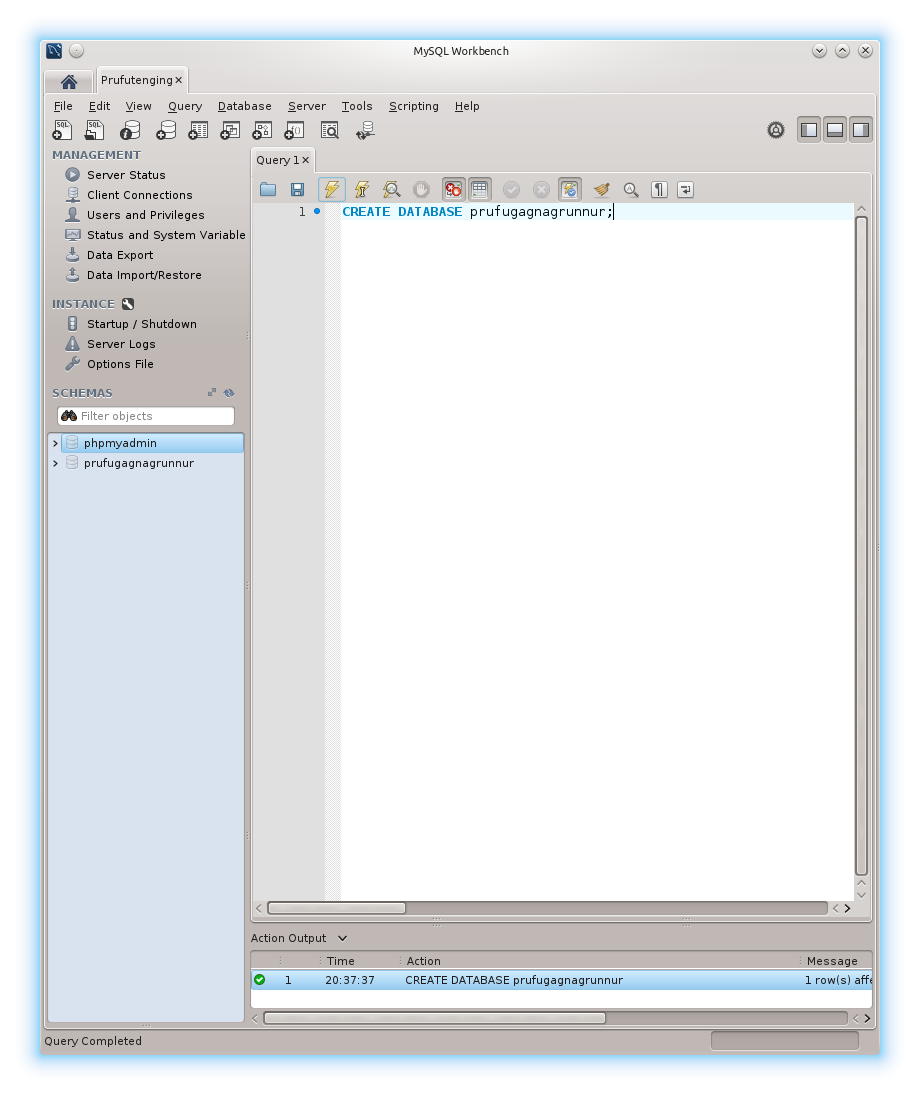
\includegraphics[width=0.8\linewidth]{myndir/workbench-create-db}
\end{figure*}

\begin{figure*}
\caption[Ný tafla]{Ný tafla búin til með MySQL Workbench. Skipunin er slegin inn í aðalgluggann og keyrð með ``eldingarhnappnum'' eins og skipunin á mynd \ref{mynd:workbench-create-db}.}
\label{mynd:workbench-create-table}
\centering
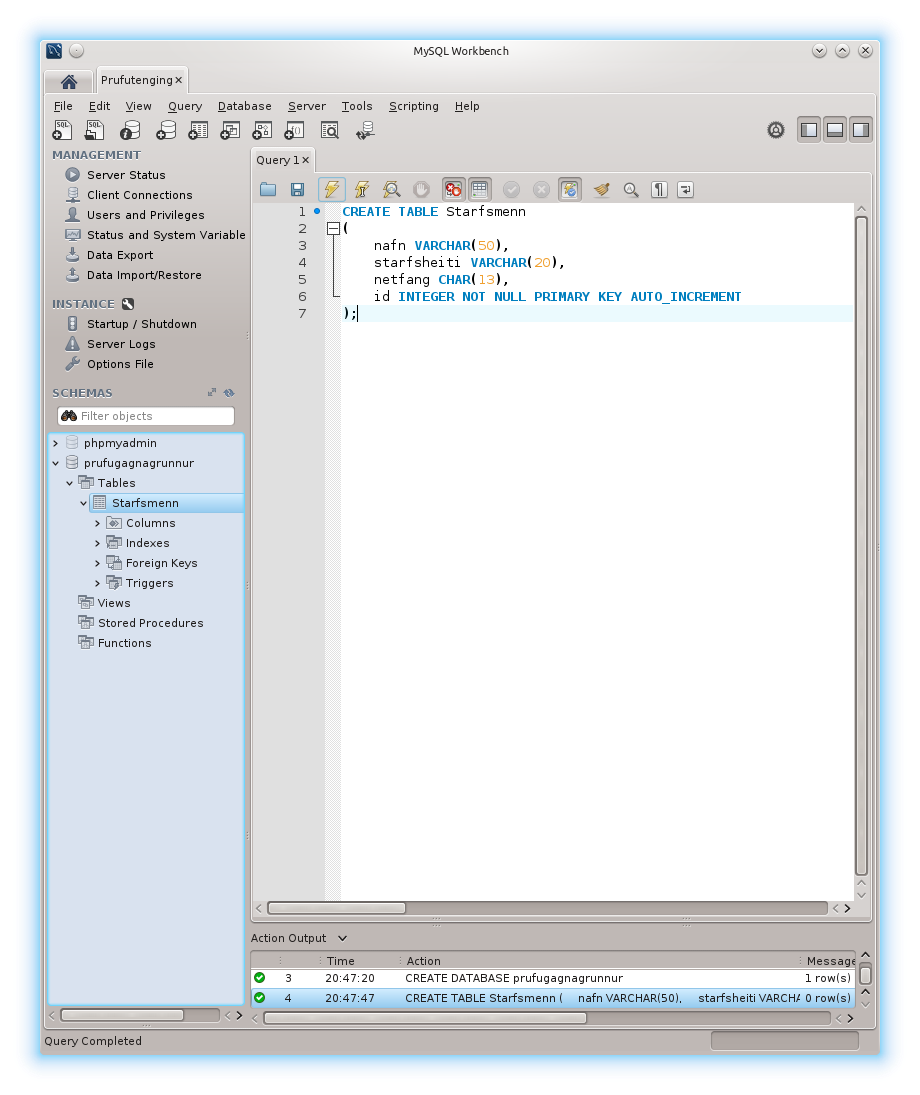
\includegraphics[width=0.8\linewidth]{myndir/workbench-create-table}
\end{figure*}

\section{Yfirlit}
Í þessum kafla fengum við örstutta kynningu því hvernig SQL-gagnagrunnar eru uppbyggðir og hvernig við getum átt samskipti við þá. 

Helstu atriðin eru:
\begin{itemize}
 \item Gögn í SQL-gagnagrunni má líta á sem línur í töflum.
 \item SQL-skipanir eru notaðir til að skilgreina töflur og setja gögn í þær.
 \item Fyrirspurnir eru notaðar til að sækja gögn úr gagnagrunnum. Fyrirspurnir eru ákveðin gerð SQL-skipana.
 \item SQL-skipanir má keyra úr aðalglugga MySQL Workbench.
\end{itemize}
Athugum að við höfum ekki farið yfir uppbyggingu skipananna. Það að læra á skipanirnar sjálfar er viðfangsefni næstu kafla.